\documentclass[border=3pt]{standalone}
% Preâmbulo compartilhado pelos diagramas TikZ da aula
\usepackage[T1]{fontenc}
\usepackage[utf8]{inputenc}
\usepackage{lmodern}
\usepackage{amsmath}
\usepackage{xcolor}
\usepackage{tikz}
\usetikzlibrary{arrows.meta,angles,quotes,decorations.pathmorphing,calc,
                positioning,shapes.geometric,backgrounds,fit}

% Paleta (mesma dos SVGs originais)
\definecolor{dblue}{HTML}{2A5B8C}
\definecolor{dorange}{HTML}{B3541E}
\definecolor{dgreen}{HTML}{4A7C59}
\definecolor{dred}{HTML}{9C4B4B}
\definecolor{dcream}{HTML}{F4F1EA}
\definecolor{dshade}{HTML}{DDD7C9}

% Estilos comuns (prefixo d... para não colidir com chaves internas do pgf)
\tikzset{
  >={Stealth[length=2mm]},
  dguide/.style={gray!55, dashed, line width=0.4pt},
  daxis/.style={gray!60, line width=0.7pt, ->},
  dbody/.style={fill=black!3, draw=black!80, line width=1pt},
  dacc/.style={draw=dblue, line width=1pt},
  dlbl/.style={black!55, font=\small},
  dsub/.style={black!45, font=\footnotesize},
  dstate/.style={circle, draw=black!80, fill=dcream, line width=1pt,
                 minimum size=17mm, font=\large, inner sep=1pt},
  dobs/.style={circle, draw=black!80, fill=dshade, line width=1pt,
               minimum size=14mm, font=\large, inner sep=1pt},
  dbox/.style={rounded corners=2pt, draw=black!80, fill=dcream, line width=1pt,
               align=center, inner sep=6pt},
  dtrans/.style={->, dblue, line width=1pt},
  dmeas/.style={->, dorange, line width=1pt},
}

\begin{document}
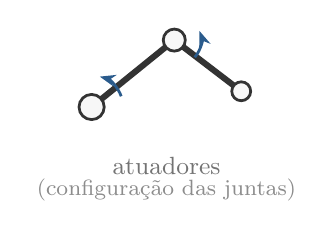
\begin{tikzpicture}[scale=1]

  \coordinate (j1) at (0,0);
  \coordinate (j2) at (1.05,0.85);
  \coordinate (j3) at (1.9,0.2);

  % elos
  \draw[black!80, line width=2.2pt, line cap=round] (j1) -- (j2) -- (j3);

  % juntas
  \foreach \p/\r in {j1/0.16, j2/0.14, j3/0.12}
    \fill[dbody] (\p) circle (\r);

  % arcos indicando rotação das juntas
  \draw[dacc, ->] ([shift=(20:0.4)]j1) arc (20:75:0.4);
  \draw[dacc, ->] ([shift=(-40:0.34)]j2) arc (-40:20:0.34);

  % legenda
  \node[dlbl]    at (0.95,-0.75) {atuadores};
  \node[dsub] at (0.95,-1.05) {(configuração das juntas)};

\end{tikzpicture}
\end{document}
